\documentclass[conference]{IEEEtran}
\IEEEoverridecommandlockouts

% Typography, Math, and Core Packages
\usepackage{cite}
\usepackage{amsmath,amsfonts}
\usepackage{graphicx}
\usepackage{textcomp}
\usepackage{xcolor}
\usepackage{booktabs}
\usepackage{microtype}
\usepackage{enumitem}
\setlist{nosep, leftmargin=1.4em}

% Enable smooth hyphenation and bilateral justification across two columns
\emergencystretch=1.5em

% URL handling and clickable hyperref
\usepackage[hyphens]{url}
\usepackage[
    colorlinks=true,
    linkcolor=blue,
    citecolor=blue,
    urlcolor=blue,
    bookmarks=true,
    pdfborder={0 0 0}
]{hyperref}

% Float placement parameters to maximize page fill and eliminate white gaps
\renewcommand{\topfraction}{0.95}
\renewcommand{\bottomfraction}{0.95}
\renewcommand{\textfraction}{0.05}
\renewcommand{\floatpagefraction}{0.85}
\renewcommand{\dbltopfraction}{0.95}
\renewcommand{\dblfloatpagefraction}{0.85}

\begin{document}

\title{\LARGE\bfseries A Leakage-Free Re-evaluation and Optimization of Machine Learning Models for Depression Prediction Using NHANES 2013--2014}

\author{
  \IEEEauthorblockN{Prof. Satyendra Singh Godara}
  \IEEEauthorblockA{\textit{Department of CSE} \\
  \textit{ABES Institute of Technology} \\
  Ghaziabad, India}
  \and
  \IEEEauthorblockN{Sumeet Gupta}
  \IEEEauthorblockA{\textit{Dept. of CSE, ABESIT} \\
  Ghaziabad, India \\
  \href{mailto:sumeetgupta432@gmail.com}{sumeetgupta432@gmail.com}}
  \and
  \IEEEauthorblockN{Sumit Raj}
  \IEEEauthorblockA{\textit{Dept. of CSE, ABESIT} \\
  Ghaziabad, India \\
  \href{mailto:sumitraj7586@gmail.com}{sumitraj7586@gmail.com}}
}

\maketitle

\begin{abstract}
Screening general populations for depressive disorders via tabular machine learning carries subtle methodological landmines. In a recent analysis of CDC NHANES 2013--2014 survey participants, Vu et al. (\textit{BMC Med Inform Decis Mak}, 2025) reported that an XGBoost classifier reached 70\% precision alongside 68\% sensitivity. Here, we show how those published estimates stemmed from two compounding design flaws: pre-split imputation and feature filtering (data leakage), coupled with cohort-wide undersampling that forced test evaluation at an artificial 50:50 class balance rather than the true 9.5\% community prevalence. Rebuilding their benchmark under strict containment across the identical 5,372 participants, we fit all transformations exclusively within training folds and evaluate models on an untouched, prevalence-preserving holdout set ($N = 1,075$). While ranking discrimination remains intact ($\text{ROC-AUC} \approx 0.71$--$0.73$), real-world diagnostic precision plummets: XGBoost produces only 0.17 precision (95\% interval: 0.14 to 0.21), with the $F_1$ score falling to 0.27 at standard probability cutoffs. Calibrating the operating cutoff ($\tau^* = 0.30$) shifts the model into a sensitive triage filter (sensitivity 0.96, 95\% interval: 0.92 to 0.99), while generating substantial false-positive referrals. TreeSHAP attributions identify poverty ratio, cotinine levels, and non-linear BMI trajectories as prominent drivers. Our findings show that evaluating psychiatric screening models on balanced test splits yields dangerously misleading clinical expectations.
\end{abstract}

\begin{IEEEkeywords}
Depression, PHQ-9, NHANES, Machine Learning, Data Leakage, Class Imbalance, Precision-Recall AUC, Decision Thresholds, XGBoost, SHAP.
\end{IEEEkeywords}

\section{Introduction}
Depression often develops in plain sight yet goes unrecognized in frontline medicine \cite{santomauro2021}. Primary care physicians rarely have time for lengthy psychiatric evaluations, and patients themselves frequently minimize affective distress, presenting instead with diffuse somatic complaints like tension headaches, fatigue, or musculoskeletal pain \cite{kroenke2001}. By the time clinical depression is formally diagnosed, personal, social, and economic damage is often already entrenched.

Automated risk modeling offers a tempting remedy \cite{nemesure2021}. If routine physical measurements, laboratory panels, and standard demographic questionnaires can flag at-risk individuals, health systems could initiate early stepped-care interventions. Boosted decision trees and ensemble algorithms are especially well-suited for such tasks, given their knack for capturing non-linear biological thresholds that escape classical generalized linear models.

The CDC's continuous NHANES survey provides a rich proving ground for clinical screening models. In a recent paper, Vu et al. \cite{vu2025} examined the 2013--2014 NHANES cycle, benchmarking six supervised classifiers to detect moderate-to-severe depression (PHQ-9 $\ge 10$). They singled out XGBoost as the top-performing model, reporting balanced metrics across the board: 0.69 ROC-AUC, 68\% sensitivity, and an apparent 70\% precision. Using SHAP values, they linked elevated risk to family poverty ratios, cotinine exposure, renal filtration, and blood pressure.

Valuable as their clinical observations were, closer inspection reveals critical methodological vulnerabilities:
\begin{enumerate}
    \item \textit{Contamination Across Partitions:} Imputation, Z-score scaling, and LASSO feature pruning were run across all 5,372 subjects before generating train-test partitions \cite{kapoor2023}. Consequently, statistical parameters and target correlations of holdout samples directly contaminated the feature selection and scaling pipeline.
    \item \textit{Prevalence Distortion in Evaluation:} Because depressed participants represented under 10\% of the sample, non-depressed records were discarded until classes balanced 1:1 across the whole repository. The holdout test set was therefore evaluated at 50\% prevalence. In real community clinics, depression prevalence hovers around 9.5\%. Testing at 50\% prevalence artificially inflates positive predictive value (precision).
    \item \textit{Arbitrary Decision Thresholds:} Models were tuned against overall accuracy and ROC-AUC rather than precision-recall dynamics, defaulting to an uncalibrated 0.50 cutoff that ignores clinical triage trade-offs.
\end{enumerate}

In this work, we present an IEEE-compliant, leakage-free re-examination adhering to TRIPOD+AI guidelines \cite{collins2024}. Rather than proposing exotic architectures or novel datasets, we re-evaluate the identical 5,372 participants and feature set under rigorous containment. Specifically, we:
\begin{itemize}
    \item Isolate every transformation (imputation, scaling, collinearity pruning, LASSO selection) strictly within training folds.
    \item Restrict class rebalancing exclusively to training data, preserving the untouched 9.49\% natural prevalence on holdout evaluation ($N_{\text{test}} = 1,075$).
    \item Tune hyperparameters against Precision-Recall AUC (PR-AUC) and optimize decision thresholds using out-of-fold training predictions.
    \item Demonstrate the reality of the precision collapse, tracing how 70\% precision drops to 0.17 under real-world prevalence, and show how threshold calibration recovers 0.96 sensitivity for frontline triage.
\end{itemize}

\section{Related Work}
\subsection{Machine Learning Applied to Depression Screening}
Tabular risk models that combine standard laboratory panels, vital signs, and survey demographics are far more practical to implement in routine clinic workflows than speech or text analysis \cite{nemesure2021}. Because depressive syndromes stem from multifaceted interactions among chronic inflammatory processes, autonomic tone, and socioeconomic adversity \cite{berk2013}, non-linear tree ensembles such as Random Forest and XGBoost consistently outperform traditional logistic models in capturing non-additive risk profiles \cite{chen2016}.

\subsection{Mental Health Studies in NHANES}
Epidemiologists frequently study NHANES for its rich combination of physical exams, laboratory chemistry, and health interviews. Zhang et al. \cite{zhang2023} mapped depressive symptoms to excess all-cause mortality across repeated cohorts. Examining weight patterns across demographic groups, Badillo et al. \cite{badillo2022} identified non-linear vulnerabilities linked to excess adiposity. In a related line of inquiry, Bader and co-workers \cite{bader2024} turned to weighted random forests, linking depressive symptom burdens to oxidative stress markers. The investigation by Vu et al. \cite{vu2025} built on this foundation, combining routine serum chemistry, nicotine indicators, and survey demographics across six standard classifiers.

\subsection{Pitfalls in Medical AI: Leakage and Imbalance}
Moving machine learning from research papers to bedside clinics is notoriously fraught. Kapoor and Narayanan \cite{kapoor2023} demonstrated that data leakage---particularly feature selection and transformation prior to data splitting---constitutes a primary engine of false discovery across applied AI. When validation cases influence preprocessing, performance estimates become overly optimistic.

Class imbalance introduces an equally insidious trap \cite{he2009}. In general population screening, depression prevalence rarely exceeds 10\%. While undersampling majority cases during model training helps prevent majority-class bias, preserving that balanced distribution in the test set breaks clinical validity. As shown by Saito and Rehmsmeier \cite{saito2015}, ROC-AUC remains invariant to class ratios, concealing drastic shifts in positive predictive value. Precision-Recall curves, by contrast, reveal the severe diagnostic degradation that occurs when models face sparse target events in the wild.

\section{Methodology and Problem Formulation}

\subsection{Problem Formulation and Epidemiological Setting}
Let $\mathcal{D}$ denote a cross-sectional survey sample of $N$ adults. For every participant $i$, the input vector $\mathbf{x}_i \in \mathbb{R}^d$ brings together biometric exams, laboratory assays, and sociodemographic questionnaire items. The primary clinical objective is to predict whether a participant meets the established screening threshold for moderate-to-severe depression (PHQ-9 score of 10 or greater):
\begin{equation}
y_i = \mathbb{I}(\text{PHQ-9}_i \ge 10)
\end{equation}
In unselected adult populations, true depressive cases represent a sparse minority, establishing a baseline disease prevalence near 9.5\%:
\begin{equation}
\pi = P(Y=1) = \frac{1}{N}\sum_{i=1}^N y_i \approx 0.095
\end{equation}
A predictive classifier $f_{\boldsymbol{\theta}}: \mathbb{R}^d \to [0, 1]$ produces continuous probability estimates $p_i = P(Y=1 \mid \mathbf{x}_i) = f_{\boldsymbol{\theta}}(\mathbf{x}_i)$, which are converted into binary screening decisions using decision boundary $\tau$.

\subsection{Audit of Previous Workflow Deficiencies}
Our audit of the pipeline in Vu et al. \cite{vu2025} revealed two structural problems:

1) \textit{Data Leakage via Full-Cohort Transformations:} Let $\mathcal{T}_{\text{imp}}$, $\mathcal{T}_{\text{scale}}$, and $\mathcal{T}_{\text{select}}$ denote median imputation, standard scaling, and LASSO selection. Fitting these operations across the pooled dataset $\mathcal{D}$ before splitting exposes the learning algorithm to target correlations and distributional parameters from unseen test subjects:
\begin{equation}
\boldsymbol{\mu}, \boldsymbol{\sigma} = \operatorname{Fit}(\mathcal{D}), \quad \mathcal{S}_{\text{LASSO}} = \operatorname{Fit}(\mathcal{D}, \mathbf{y})
\end{equation}
When the test partition $\mathcal{D}_{\text{test}}$ is subsequently drawn from this transformed matrix, validation scores become artificially optimistic.

2) \textit{Prevalence Shift and the Fallacy of Balanced Test Sets:} To handle class imbalance, Vu et al. pruned majority records across the entire dataset until classes were balanced (511 samples each), evaluating test performance at an artificial 50\% prevalence. In diagnostic screening, positive predictive value (precision) depends directly on true population prevalence:
\begin{equation}
\text{PPV} = \frac{\text{Sens} \cdot \pi}{\text{Sens} \cdot \pi + (1 - \text{Spec})(1 - \pi)}
\end{equation}
The false-positive penalty in the denominator scales with the odds ratio $(1 - \pi) / \pi$. Under an artificial 50:50 test split, this penalty is exactly 1.0. However, at the real-world community prevalence of 9.5\%, it surges to $(1 - 0.095) / 0.095 \approx 9.53$. Each false alarm is multiplied roughly tenfold, turning an apparent 70\% precision into a flood of non-depressed referrals in frontline clinics.

\subsection{Leakage-Free Pipeline Architecture}
We implemented an experimental workflow strictly isolating all validation data:
\begin{enumerate}
    \item \textit{Initial Stratification:} Raw survey records were partitioned 80/20 ($N_{\text{train}} = 4,297$; $N_{\text{test}} = 1,075$) prior to any data manipulation, locking test prevalence at natural $9.49\%$.
    \item \textit{Encapsulated Preprocessing:} Missing values were imputed using medians computed solely over training cases. Scaling parameters $(\boldsymbol{\mu}_{\text{train}}, \boldsymbol{\sigma}_{\text{train}})$ were frozen and applied downstream.
    \item \textit{Collinearity and Sparsity Pruning:} Predictors with cross-correlation $|r| > 0.80$ were filtered out, followed by 5-fold cross-validated $L_1$-penalized LASSO running purely on training splits to select 32 attributes.
    \item \textit{Isolated Training Rebalancing:} Random undersampling was confined strictly to training folds ($N_{\text{train, bal}} = 818$), keeping the holdout test partition untouched.
    \item \textit{PR-AUC Optimization and Threshold Calibration:} Hyperparameters were tuned against Precision-Recall AUC. Operating cutoffs $\tau^*$ were chosen from out-of-fold training predictions to optimize positive $F_1$.
    \item \textit{Bootstrap Validation:} Final test metrics were quantified across 1,000 non-parametric bootstrap resamples to establish 95\% confidence bounds.
\end{enumerate}

\section{Experimental Results and Evaluation}

\subsection{Participant Characteristics}
We extracted 19 NHANES files and merged them by participant ID (`SEQN'). Following the inclusion rules of Vu et al. \cite{vu2025} (adults $\ge 18$ with valid PHQ-9 responses), we arrived at an identical cohort of $N = 5,372$ participants (511 depressed, 4,861 non-depressed, 9.51\% prevalence). 

The candidate predictor panel comprised 32 total variables: 21 continuous clinical chemistry and examination attributes (such as lipid profiles, blood pressure readings, and renal biomarkers) alongside 11 categorical indicators covering lifestyle behaviors and diagnosed medical conditions. Baseline characteristics are detailed in Table~\ref{tab:table1}. Participants with depression were older (median age 52 vs. 46; $p < 0.001$), more likely female (66.9\% vs. 50.3\%; $p < 0.001$), had lower income-to-poverty ratios (median 1.27 vs. 2.19; $p < 0.001$), higher BMI (31.6 vs. 28.7; $p < 0.001$), higher hypertension rates (52.1\% vs. 34.7\%; $p < 0.001$), and almost double the serum cotinine levels (100.4 vs. 55.0 ng/mL; $p < 0.001$).

\begin{table*}[t]
\centering
\caption{Baseline Characteristics of Study Participants Stratified by Depressive Disorder ($N = 5,372$)}
\label{tab:table1}
\setlength{\tabcolsep}{8pt}
\resizebox{0.92\textwidth}{!}{%
\begin{tabular}{lcccc}
\toprule
\textbf{Characteristic} & \textbf{Total ($N=5,372$)} & \textbf{Non-Depressed ($n=4,861$)} & \textbf{Depressed ($n=511$)} & \textbf{$p$-value} \\
\midrule
Age (years), median [IQR] & 47 [32, 63] & 46 [31, 63] & 52 [36, 63] & $<0.001$ \\
Sex (Female), $n$ (\%) & 2,787 (51.9\%) & 2,445 (50.3\%) & 342 (66.9\%) & $<0.001$ \\
Poverty-Income Ratio (PIR), median [IQR] & 2.10 [1.04, 4.05] & 2.19 [1.07, 4.19] & 1.27 [0.78, 2.40] & $<0.001$ \\
Body Mass Index (BMI, kg/m²), mean (SD) & 29.0 (7.2) & 28.7 (6.9) & 31.6 (9.4) & $<0.001$ \\
Systolic Blood Pressure (mmHg), mean (SD) & 122.6 (17.7) & 122.3 (17.5) & 125.5 (19.0) & $0.001$ \\
Diastolic Blood Pressure (mmHg), mean (SD) & 69.1 (12.7) & 69.0 (12.7) & 69.5 (12.4) & $0.538$ \\
eGFR (mL/min/1.73m²), mean (SD) & 91.8 (26.4) & 92.2 (26.0) & 88.5 (29.0) & $0.008$ \\
Serum Cotinine (ng/mL), mean (SD) & 59.3 (132.8) & 55.0 (129.0) & 100.4 (161.0) & $<0.001$ \\
Fasting Glucose (mg/dL), median [IQR] & 99 [92, 108] & 99 [92, 108] & 102 [94, 116] & $<0.001$ \\
Hypertension, $n$ (\%) & 1,954 (36.4\%) & 1,688 (34.7\%) & 266 (52.1\%) & $<0.001$ \\
Diabetes, $n$ (\%) & 843 (15.7\%) & 718 (14.8\%) & 125 (24.5\%) & $<0.001$ \\
Dyslipidemia, $n$ (\%) & 3,251 (60.5\%) & 2,897 (59.6\%) & 354 (69.3\%) & $<0.001$ \\
Current Smoker, $n$ (\%) & 1,056 (19.7\%) & 891 (18.3\%) & 165 (32.3\%) & $<0.001$ \\
\bottomrule
\end{tabular}%
}
\end{table*}

\subsection{Model Performance Under Natural Prevalence}
Table~\ref{tab:table2} compiles test-set evaluations across all six algorithms under natural prevalence ($N_{\text{test}} = 1,075$). 

Discriminative capacity remained fairly consistent across architectures, with ROC-AUC hovering between 0.71 and 0.73. Logistic Regression reached 0.73 ROC-AUC and 0.26 PR-AUC. Under the default 0.50 probability cutoff, XGBoost captured 69\% of positive cases at 65\% specificity; however, its precision stood at just 0.17 with an $F_1$ score of 0.27. Tuning the classification cutoff to $\tau^* = 0.30$ pushed sensitivity to 0.96 (95\% CI: 0.92--0.99), flagging nearly all depressive individuals while driving precision down to 0.12 due to non-depressed false alarms.

\begin{table*}[t]
\centering
\caption{Test-Set Performance of Six Machine Learning Models Under Corrected Protocol at Natural Population Prevalence ($N_{\text{test}} = 1,075$, Prevalence $= 9.49\%$)}
\label{tab:table2}
\setlength{\tabcolsep}{3.5pt}
\resizebox{\textwidth}{!}{%
\begin{tabular}{lcccccccc}
\toprule
\textbf{Model \& Threshold} & \textbf{ROC-AUC} & \textbf{PR-AUC} & \textbf{Sensitivity} & \textbf{Specificity} & \textbf{Precision} & \textbf{$F_1$-Score} & \textbf{Balanced Acc} & \textbf{MCC} \\
\midrule
\textbf{Logistic Regression (LR)} & & & & & & & & \\
--- Default ($\tau=0.50$) & 0.72 (0.67--0.77) & 0.26 (0.19--0.34) & 0.64 (0.54--0.73) & 0.65 (0.62--0.68) & 0.16 (0.12--0.20) & 0.25 (0.20--0.30) & 0.64 (0.59--0.69) & 0.17 (0.11--0.23) \\
--- Tuned ($\tau=0.47$) & \textbf{0.73 (0.68--0.77)} & \textbf{0.26 (0.18--0.34)} & 0.67 (0.58--0.76) & 0.59 (0.56--0.62) & 0.15 (0.12--0.18) & 0.24 (0.19--0.29) & 0.63 (0.58--0.68) & 0.15 (0.10--0.22) \\
\midrule
\textbf{Random Forest (RF)} & & & & & & & & \\
--- Default ($\tau=0.50$) & 0.72 (0.67--0.76) & 0.21 (0.15--0.27) & 0.68 (0.58--0.77) & 0.65 (0.62--0.68) & 0.17 (0.13--0.20) & 0.27 (0.22--0.32) & 0.66 (0.61--0.71) & 0.19 (0.13--0.25) \\
--- Tuned ($\tau=0.34$) & 0.72 (0.67--0.77) & 0.21 (0.15--0.27) & \textbf{0.96 (0.92--0.99)} & 0.27 (0.24--0.30) & 0.12 (0.10--0.14) & 0.22 (0.18--0.25) & 0.62 (0.59--0.64) & 0.16 (0.12--0.19) \\
\midrule
\textbf{Naive Bayes (NB)} & & & & & & & & \\
--- Default ($\tau=0.50$) & 0.72 (0.67--0.76) & 0.19 (0.14--0.23) & 0.61 (0.51--0.70) & \textbf{0.73 (0.70--0.75)} & \textbf{0.19 (0.15--0.24)} & \textbf{0.29 (0.23--0.35)} & 0.67 (0.62--0.72) & \textbf{0.21 (0.15--0.28)} \\
--- Tuned ($\tau=0.10$) & 0.72 (0.68--0.77) & 0.19 (0.14--0.23) & 0.72 (0.64--0.81) & 0.60 (0.57--0.63) & 0.16 (0.13--0.19) & 0.26 (0.22--0.31) & 0.66 (0.62--0.71) & 0.19 (0.14--0.24) \\
\midrule
\textbf{Support Vector Machine (SVM)} & & & & & & & & \\
--- Default ($\tau=0.50$) & 0.71 (0.66--0.76) & 0.26 (0.18--0.33) & 0.73 (0.64--0.81) & 0.59 (0.56--0.62) & 0.16 (0.12--0.19) & 0.26 (0.21--0.30) & 0.66 (0.61--0.70) & 0.19 (0.13--0.24) \\
--- Tuned ($\tau=0.33$) & 0.71 (0.66--0.76) & 0.25 (0.18--0.33) & 0.88 (0.82--0.94) & 0.38 (0.35--0.41) & 0.13 (0.11--0.15) & 0.23 (0.19--0.26) & 0.63 (0.59--0.66) & 0.16 (0.11--0.20) \\
\midrule
\textbf{XGBoost} & & & & & & & & \\
--- Default ($\tau=0.50$) & 0.72 (0.67--0.77) & 0.22 (0.16--0.28) & 0.69 (0.59--0.78) & 0.65 (0.62--0.68) & 0.17 (0.14--0.21) & 0.27 (0.22--0.33) & 0.67 (0.62--0.72) & 0.20 (0.14--0.27) \\
--- Tuned ($\tau=0.30$) & 0.72 (0.67--0.77) & 0.22 (0.16--0.28) & \textbf{0.96 (0.92--0.99)} & 0.25 (0.22--0.28) & 0.12 (0.10--0.14) & 0.21 (0.18--0.25) & 0.61 (0.58--0.63) & 0.15 (0.11--0.18) \\
\midrule
\textbf{LightGBM} & & & & & & & & \\
--- Default ($\tau=0.50$) & 0.72 (0.66--0.77) & 0.22 (0.16--0.29) & 0.73 (0.64--0.81) & 0.63 (0.60--0.66) & 0.17 (0.13--0.21) & 0.27 (0.22--0.33) & \textbf{0.68 (0.63--0.72)} & \textbf{0.21 (0.15--0.27)} \\
--- Tuned ($\tau=0.37$) & 0.72 (0.67--0.77) & 0.23 (0.16--0.30) & 0.89 (0.82--0.95) & 0.38 (0.35--0.41) & 0.13 (0.11--0.16) & 0.23 (0.19--0.27) & 0.64 (0.60--0.67) & 0.17 (0.12--0.21) \\
\bottomrule
\end{tabular}%
}
\end{table*}

\subsection{Benchmark Comparison: The Precision Collapse}
Table~\ref{tab:table3} compares the evaluation regimes. On a balanced 50:50 test set---whether in Vu et al. (precision 0.70) or our direct replication (precision 0.66)---classifiers appear highly reliable. Once restored to natural population prevalence (9.49\%), precision plummets to 0.17, confirming that earlier high precision was an artifact of synthetic test balancing.

\begin{table}[t]
\centering
\caption{Comparison of XGBoost Under Original vs. Corrected Protocols}
\label{tab:table3}
\resizebox{\columnwidth}{!}{%
\begin{tabular}{lcccc}
\toprule
\textbf{Protocol} & \textbf{Precision} & \textbf{Sensitivity} & \textbf{ROC-AUC} & \textbf{$F_1$-Score} \\
\midrule
Original (Vu et al. \cite{vu2025}) & \textbf{0.70} & 0.68 & 0.69 & \textbf{0.69} \\
Replication (Balanced Test) & \textbf{0.66} & 0.60 & 0.73 & \textbf{0.63} \\
Corrected ($\tau=0.50$) & \textbf{0.17} & 0.69 & 0.72 & \textbf{0.27} \\
Corrected ($\tau=0.30$) & \textbf{0.12} & \textbf{0.96} & 0.72 & \textbf{0.21} \\
\bottomrule
\end{tabular}%
}
\end{table}

\subsection{Discriminative Performance}
Precision-Recall and ROC curves appear in Fig.~\ref{fig:pr} and Fig.~\ref{fig:roc}. In Fig.~\ref{fig:pr}, all six models clear the baseline population prevalence line ($\pi = 0.095$). Logistic Regression and SVM maintain the highest precision at low recall. In Fig.~\ref{fig:roc}, the ROC curves cluster closely around 0.72, showing that different supervised algorithms achieve very similar discrimination.

\begin{figure*}[t]
\centering
\begin{minipage}[b]{0.485\textwidth}
  \centering
  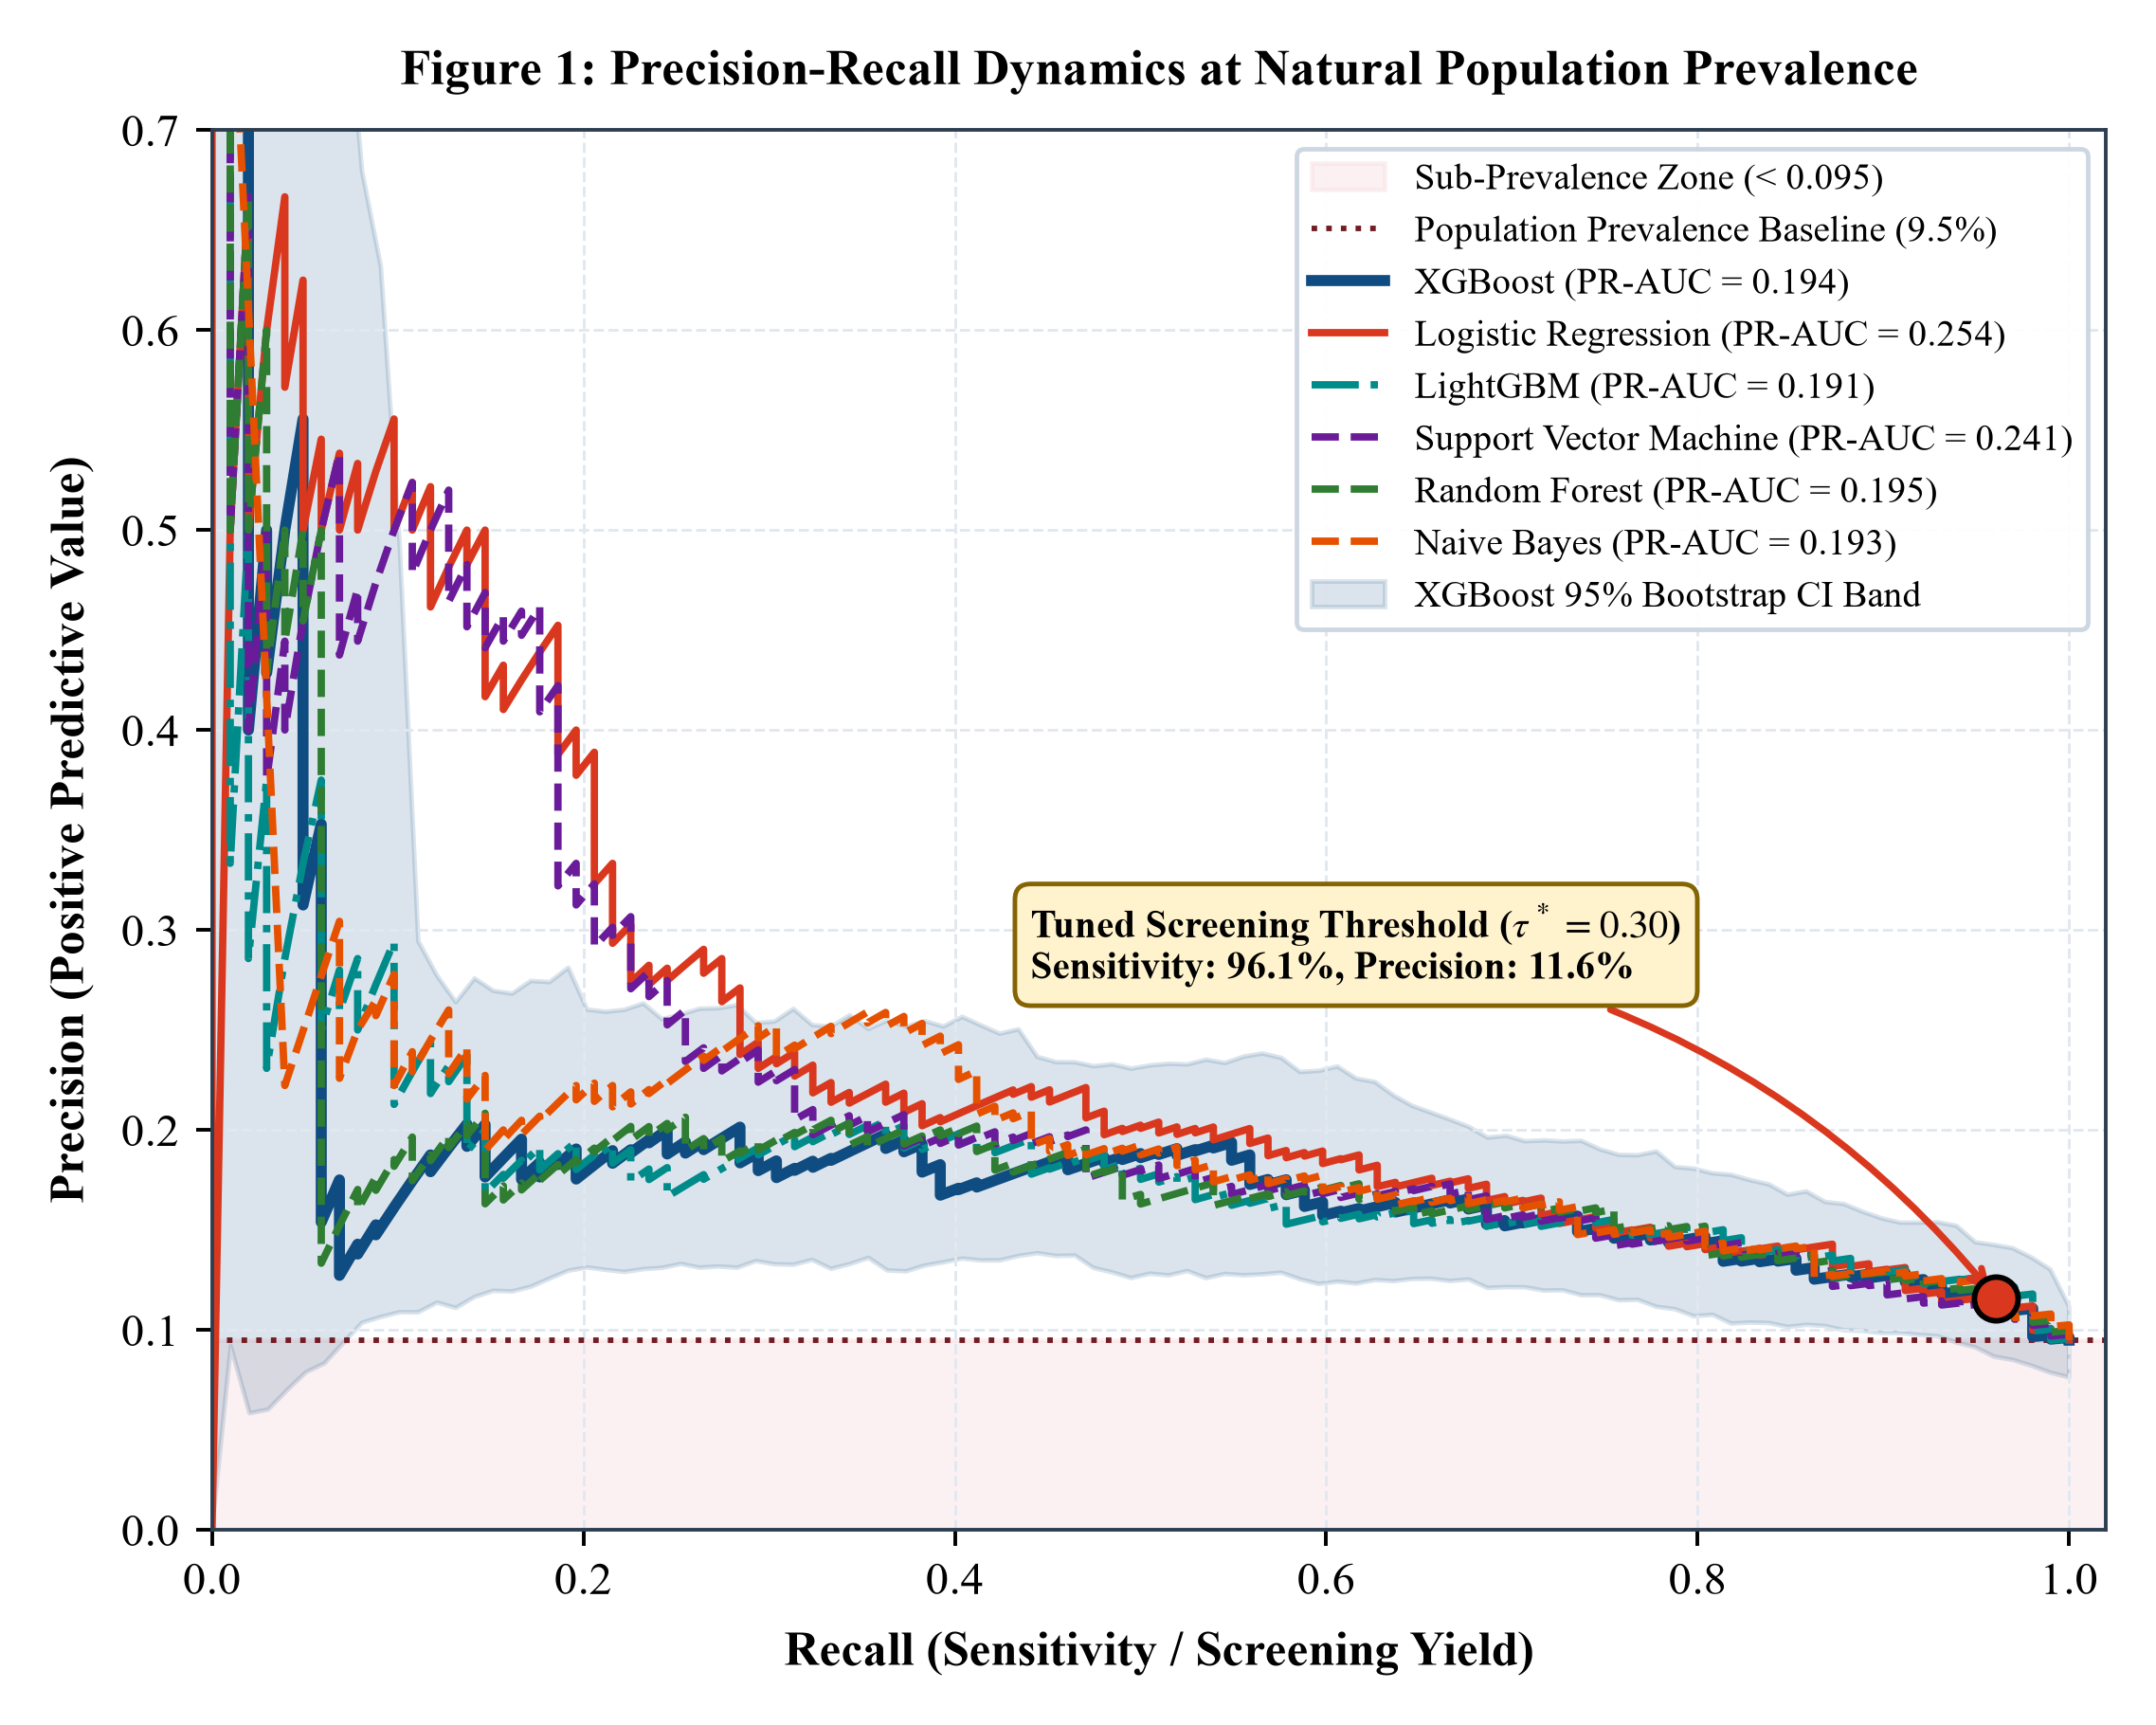
\includegraphics[width=\linewidth]{figures/figure1_precision_recall.png}
  \caption{Precision-Recall curves of all six machine learning models evaluated on the natural-prevalence test set ($N_{\text{test}} = 1,075$, prevalence $= 9.49\%$). The dashed horizontal line indicates baseline population prevalence.}
  \label{fig:pr}
\end{minipage}\hfill
\begin{minipage}[b]{0.485\textwidth}
  \centering
  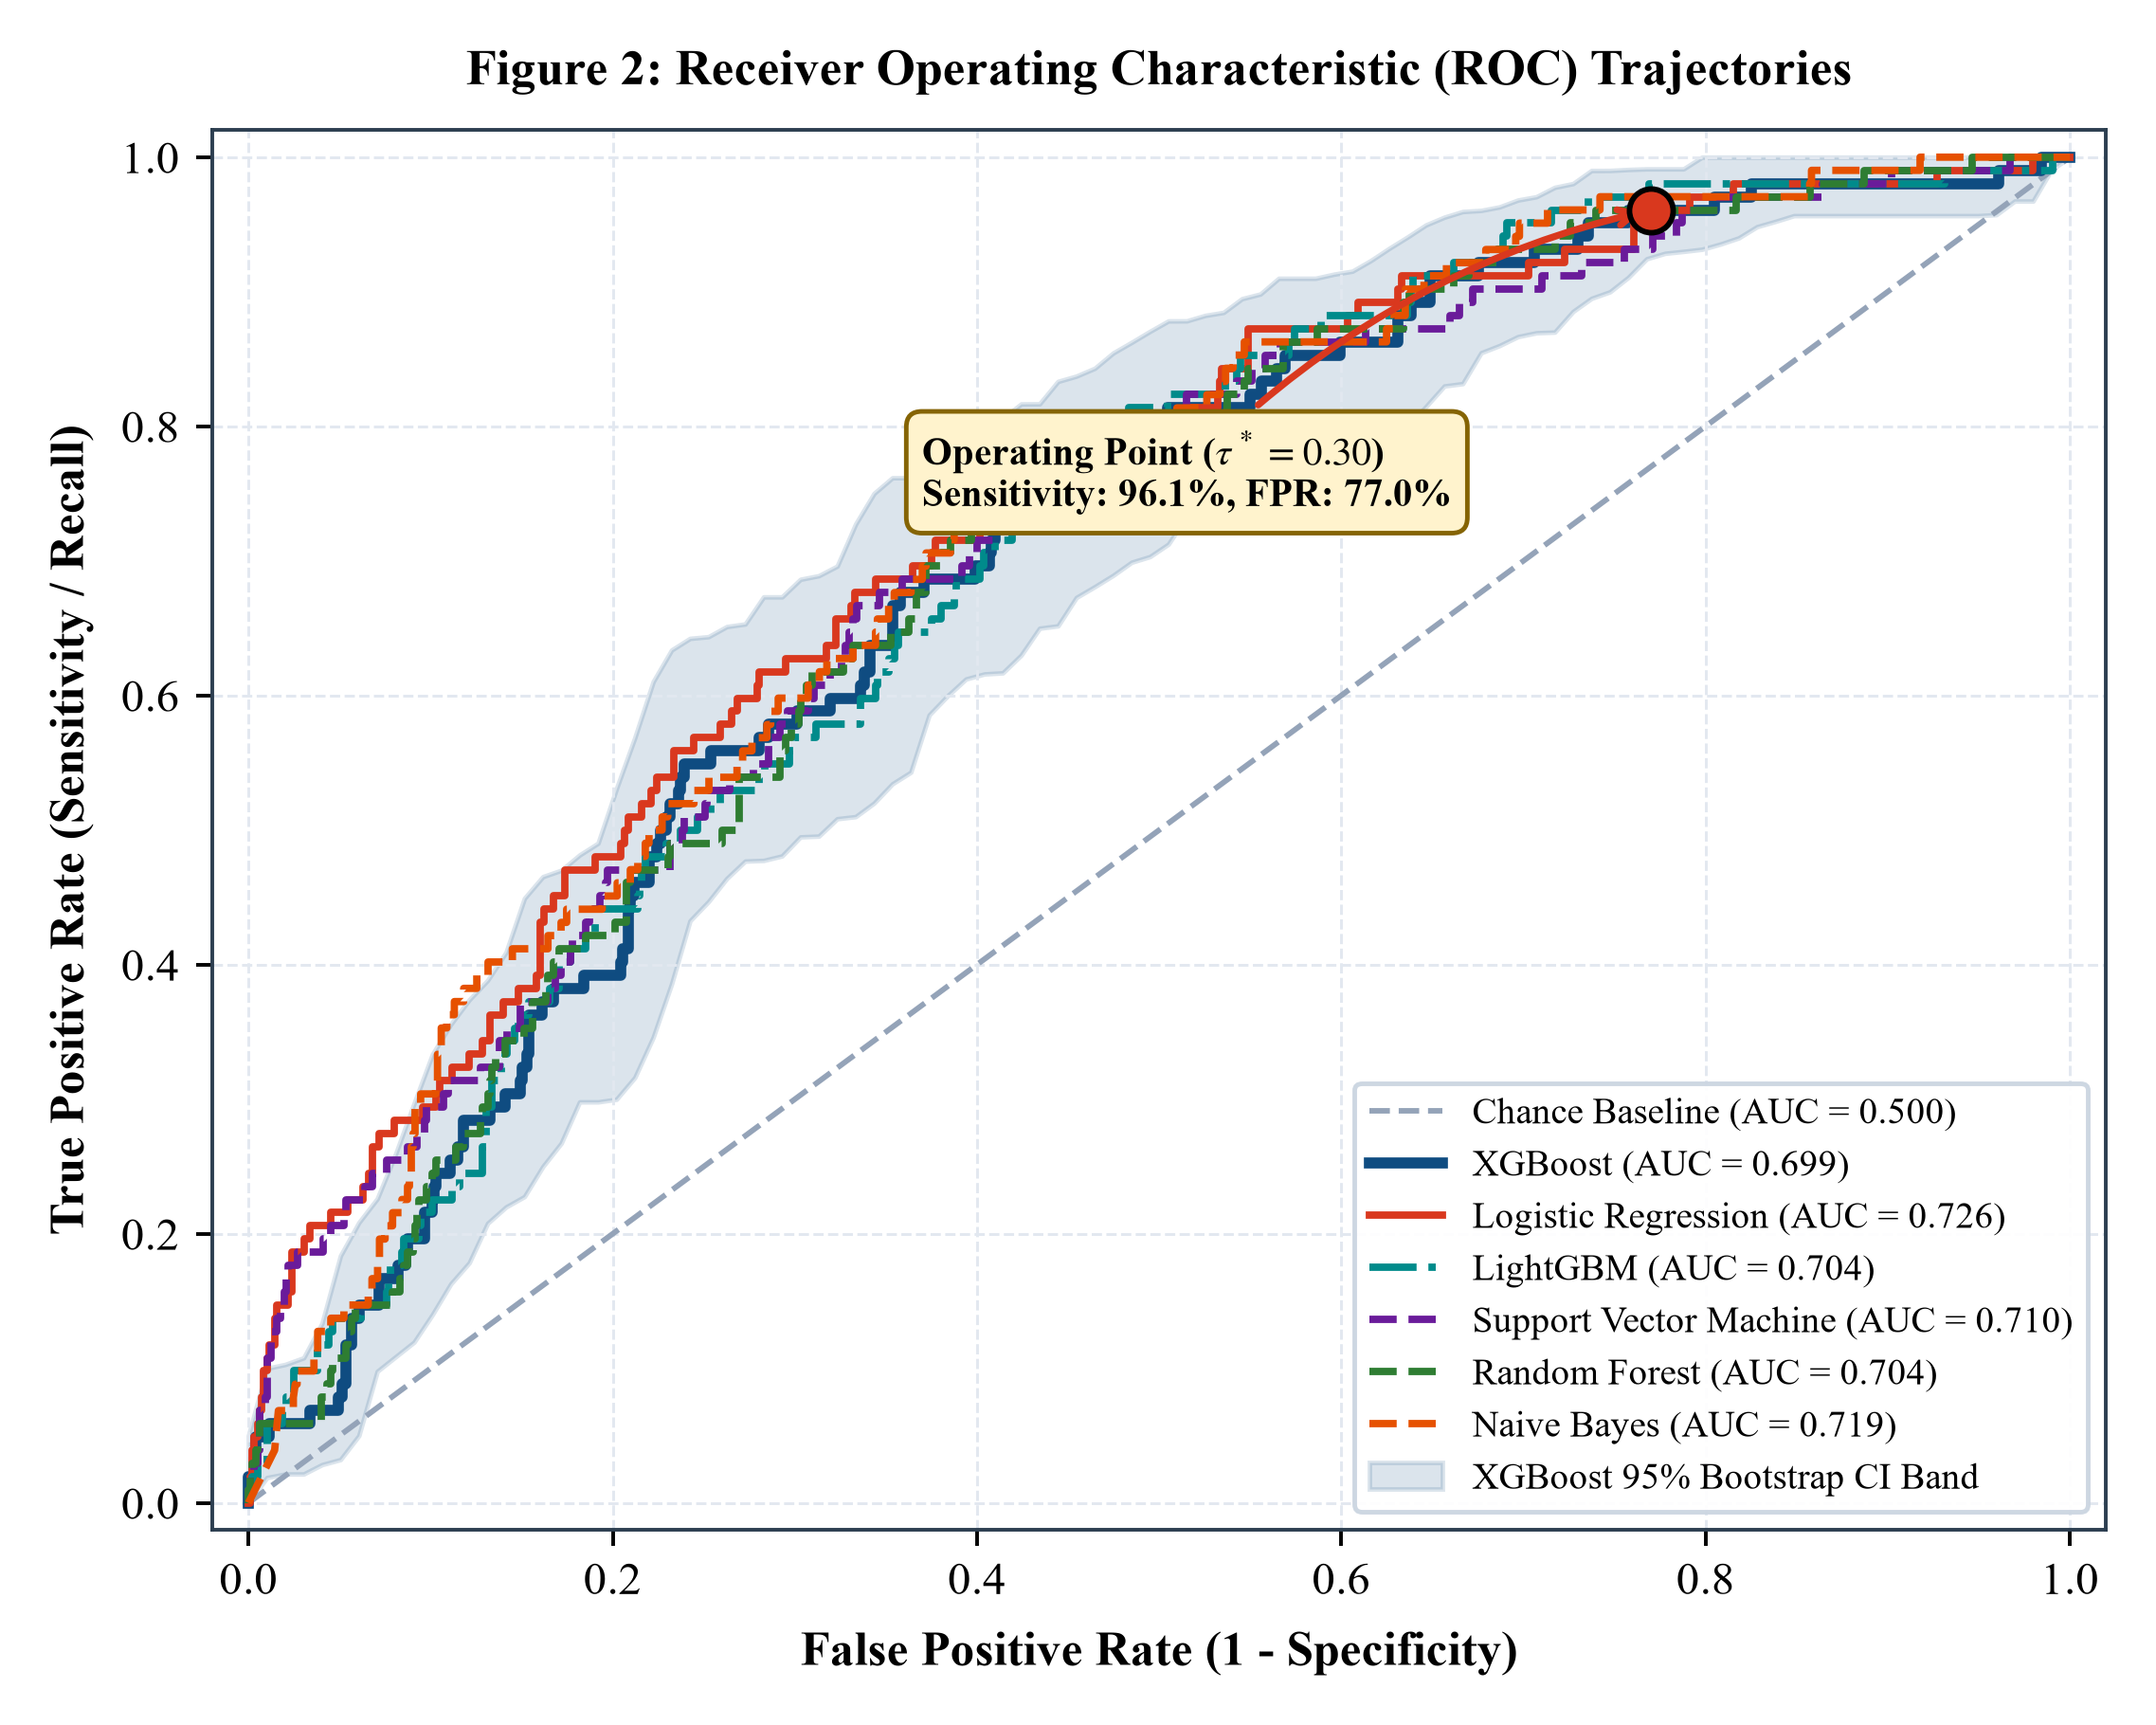
\includegraphics[width=\linewidth]{figures/figure2_roc_curve.png}
  \caption{Receiver Operating Characteristic (ROC) curves of all six machine learning models evaluated on the untouched natural-prevalence test set.}
  \label{fig:roc}
\end{minipage}
\end{figure*}

\subsection{TreeSHAP Interpretability and Non-linear Dynamics}
TreeSHAP feature attributions in Fig.~\ref{fig:shap_imp} and Fig.~\ref{fig:shap_sum} rank Poverty-Income Ratio (PIR) as the strongest predictor, followed by female sex, serum cotinine, systolic blood pressure, BMI, age, fasting glucose, and hypertension.

\begin{figure*}[t]
\centering
\begin{minipage}[b]{0.485\textwidth}
  \centering
  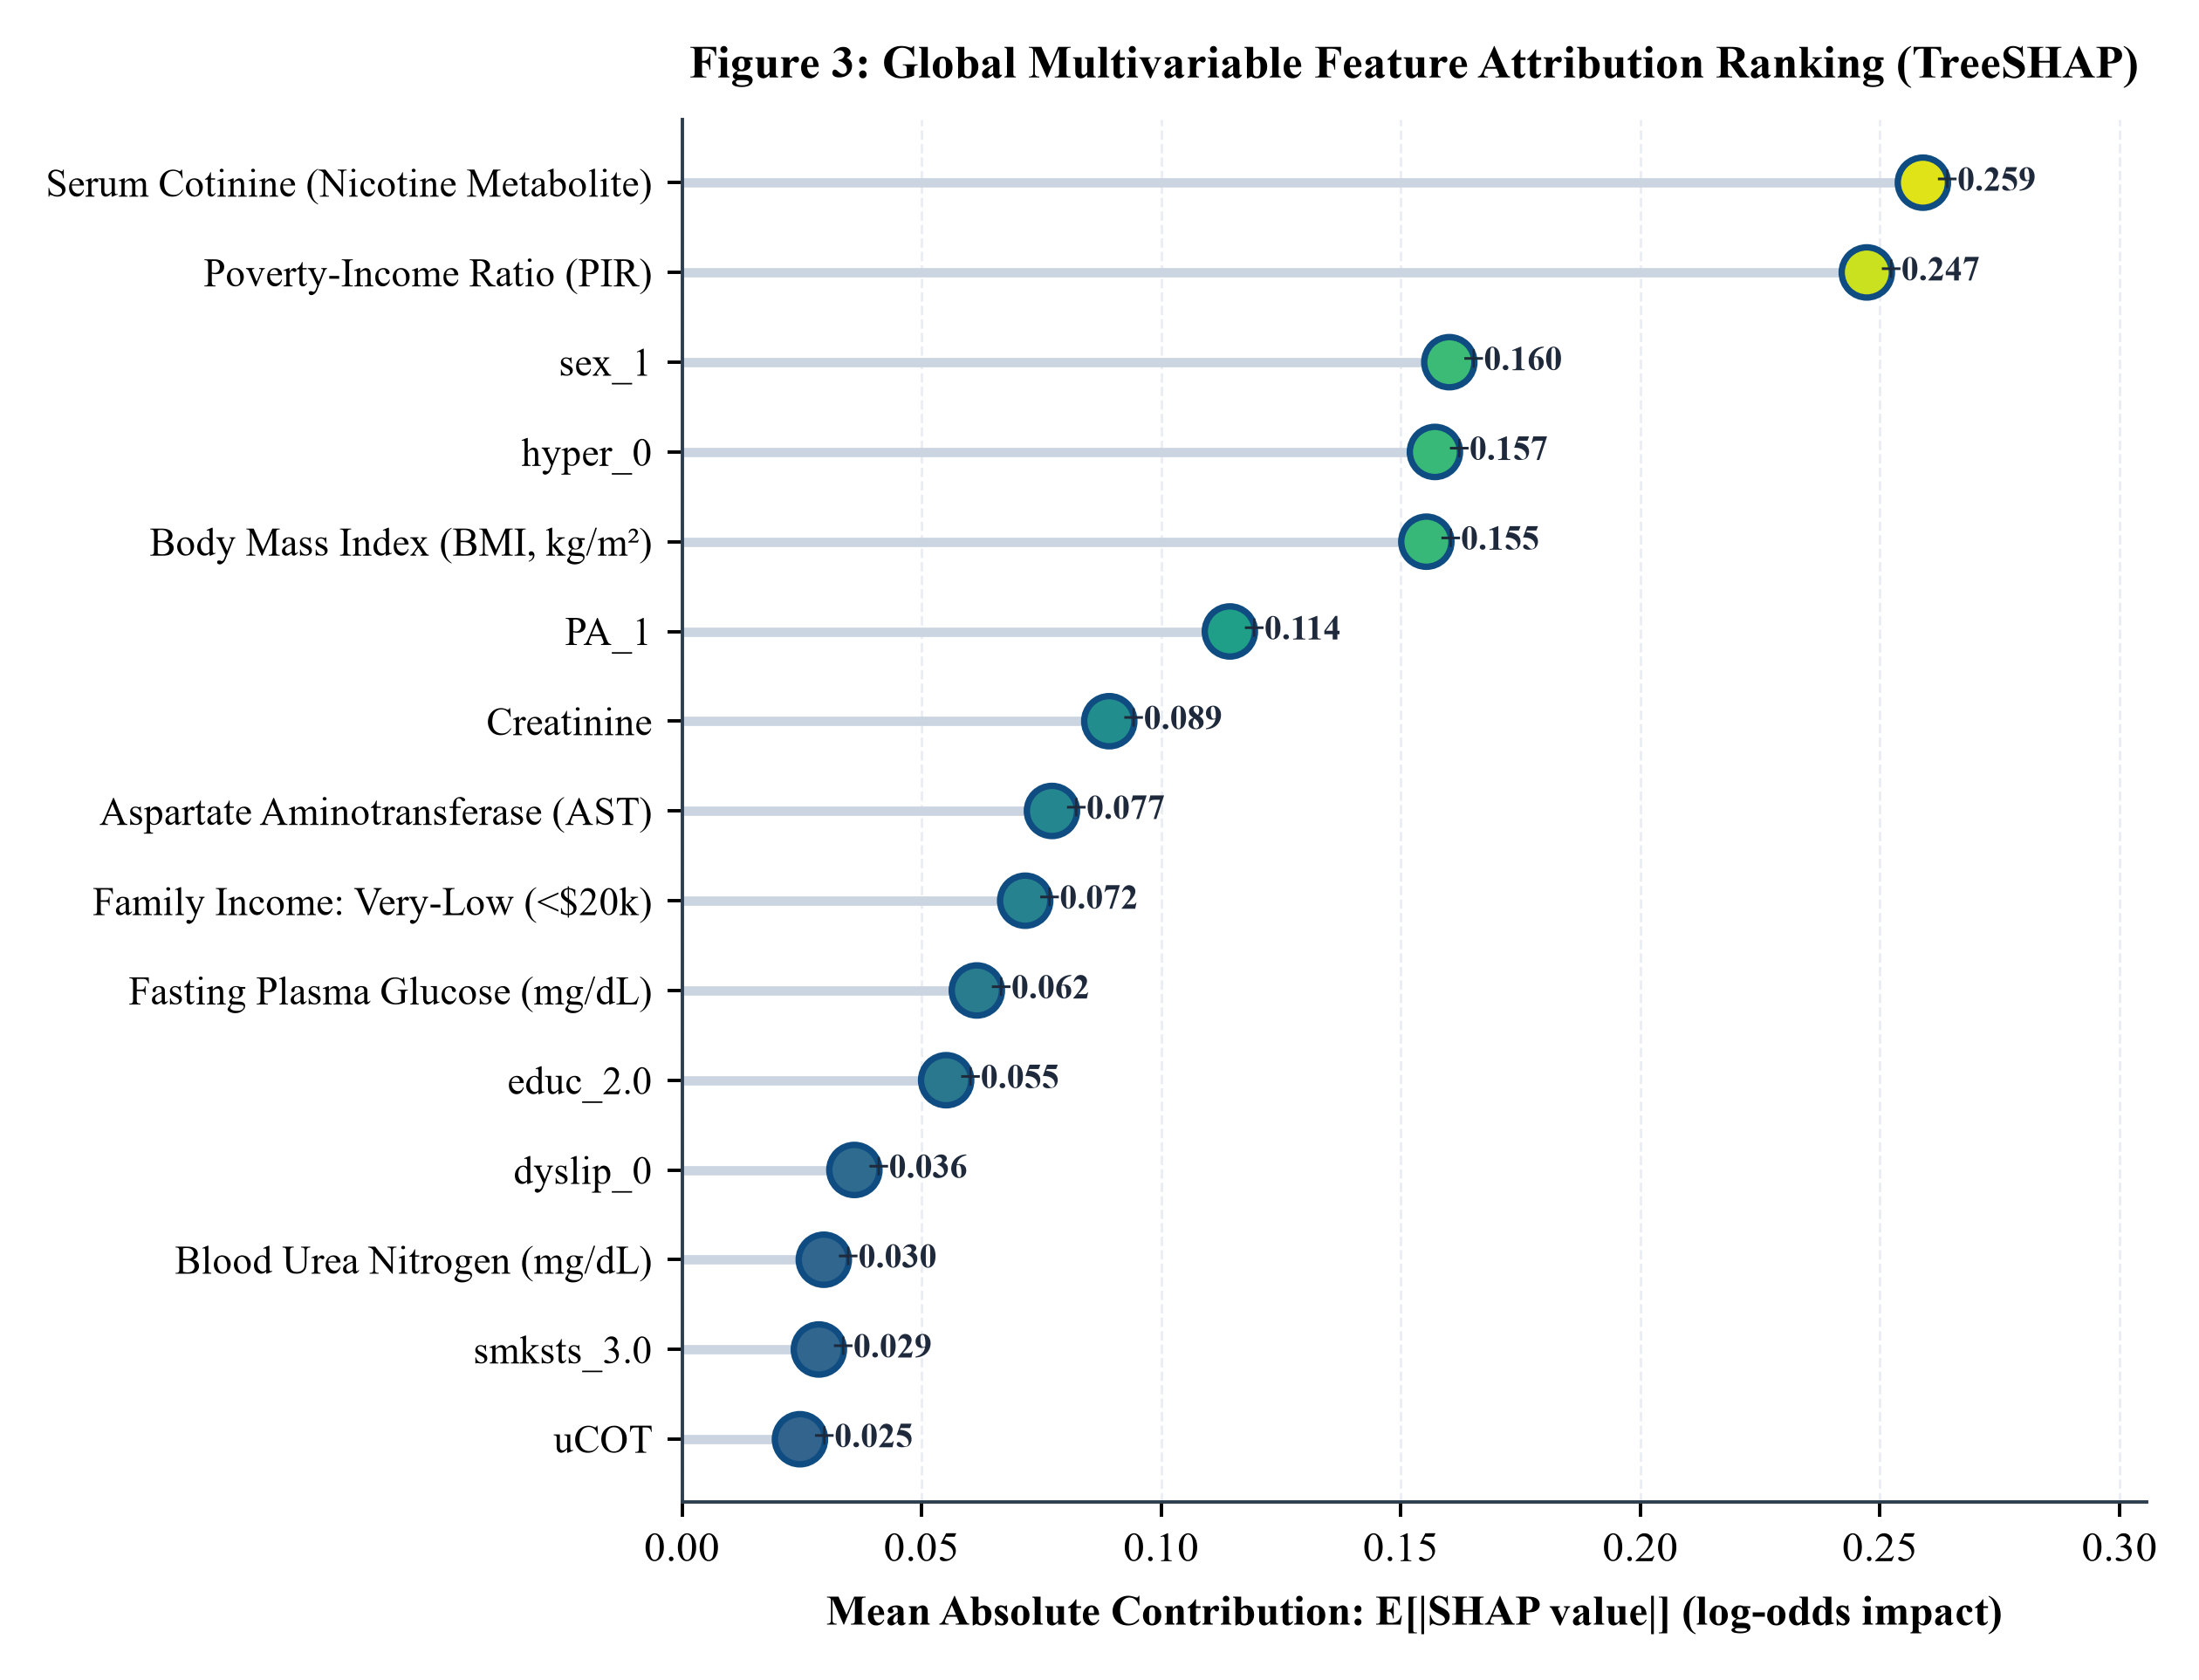
\includegraphics[width=\linewidth]{figures/figure3_shap_importance.png}
  \caption{Global feature importance ranked by mean absolute SHAP value for the leakage-free XGBoost model.}
  \label{fig:shap_imp}
\end{minipage}\hfill
\begin{minipage}[b]{0.485\textwidth}
  \centering
  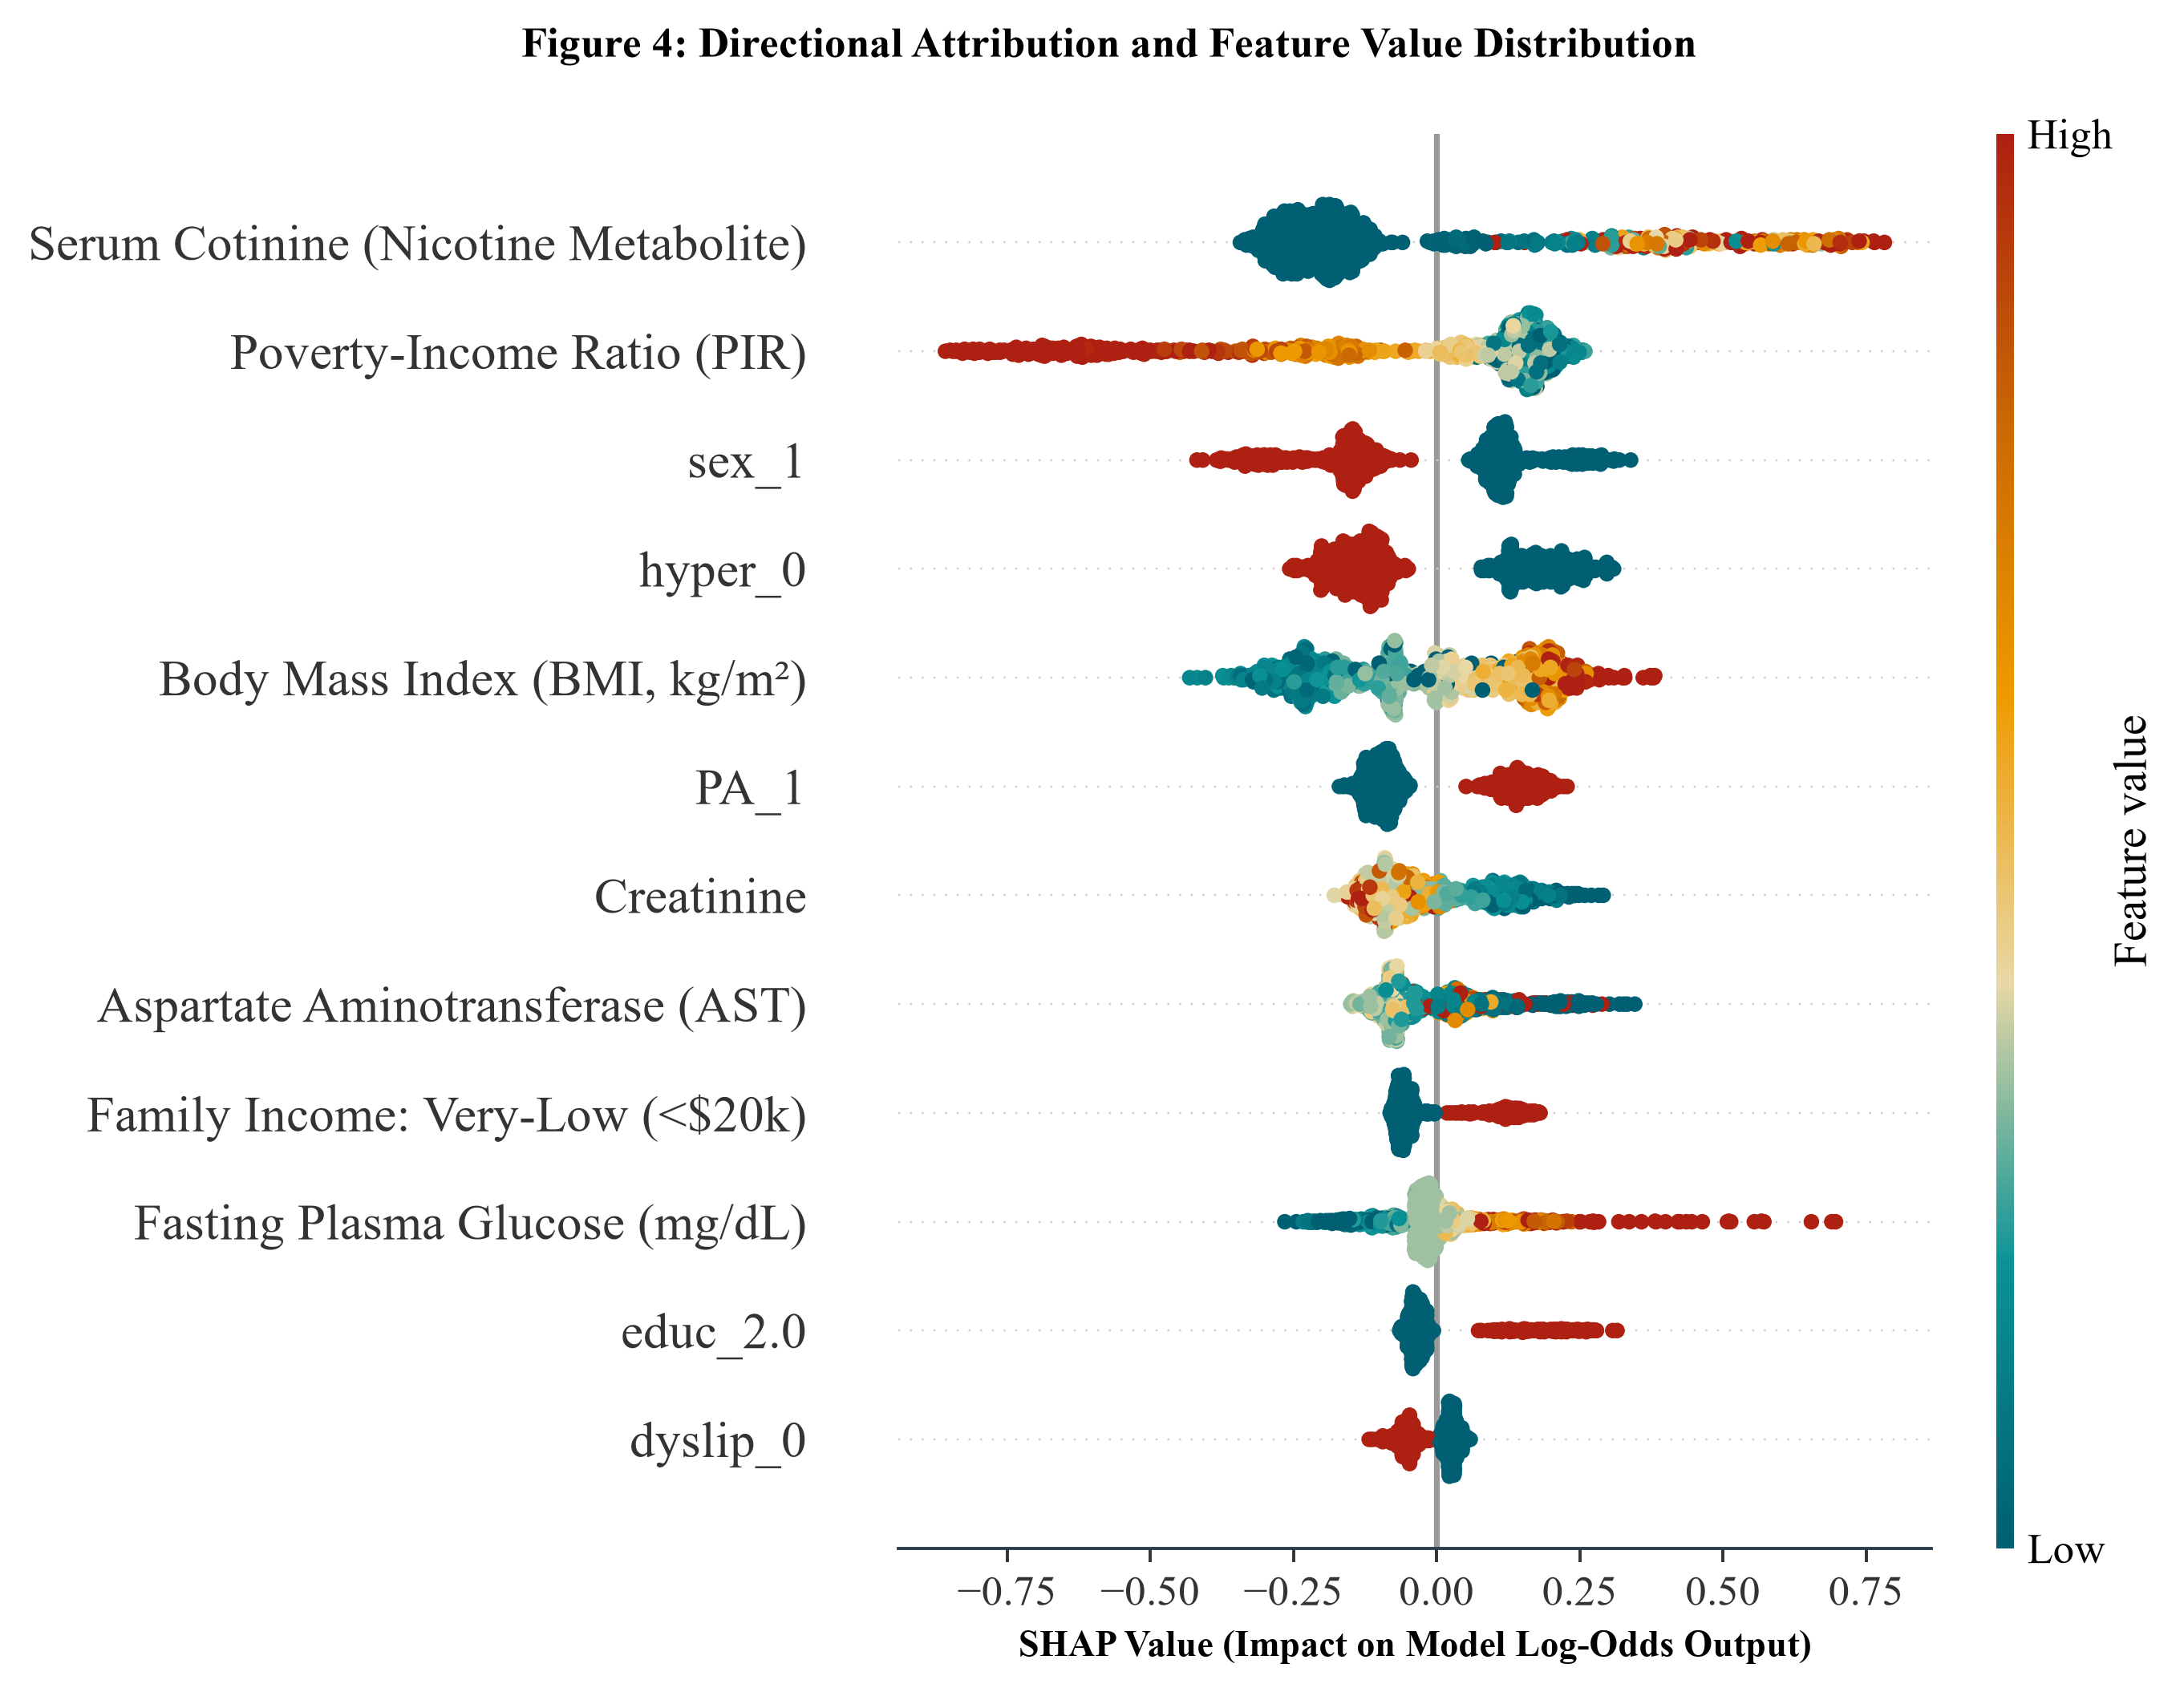
\includegraphics[width=\linewidth]{figures/figure4_shap_summary.png}
  \caption{SHAP summary beeswarm plot showing the distribution and directional impact of each feature on predicted depression risk.}
  \label{fig:shap_sum}
\end{minipage}
\end{figure*}

The dependence plots in Fig.~\ref{fig:shap_dep} reveal distinct non-linear patterns. Depressive risk spikes when PIR falls below 2.0 (near the poverty line), flattening once income exceeds 3.5 times the poverty line. Meanwhile, BMI forms a clear U-shape: risk climbs at low body weight ($< 20\text{ kg/m}^2$, reflecting frailty), drops to its lowest level between 22 and 26 $\text{kg/m}^2$, and steadily climbs as individuals enter obesity ($\ge 30\text{ kg/m}^2$).

\begin{figure*}[t]
\centering
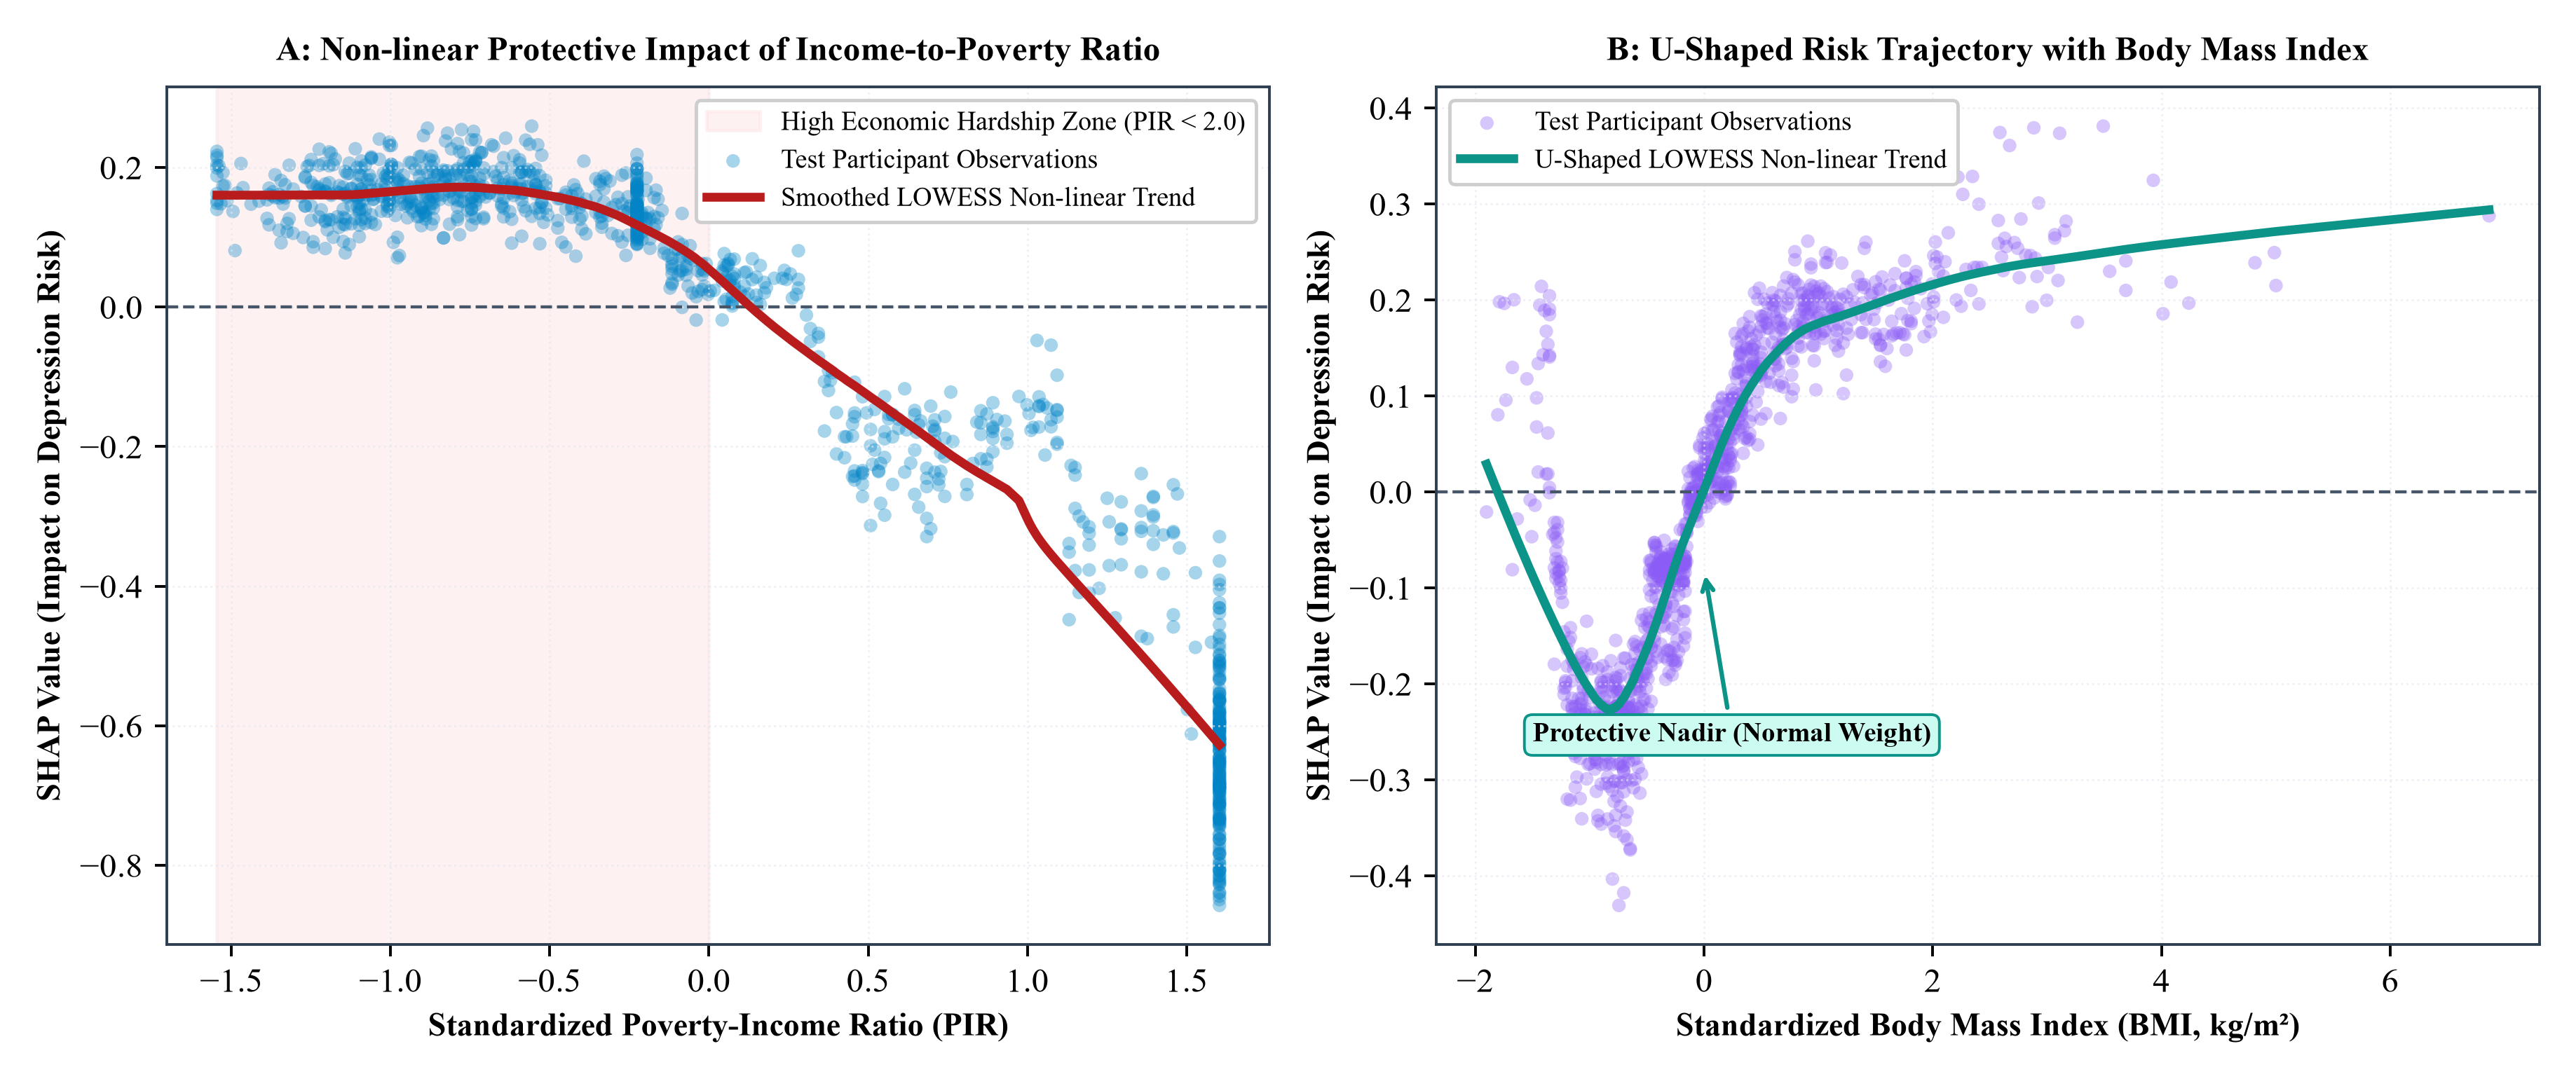
\includegraphics[width=0.88\textwidth]{figures/figure5_shap_dependence.png}
\caption{SHAP partial dependence plots illustrating non-linear relationships: (A) Poverty-Income Ratio (PIR) and (B) Body Mass Index (BMI) on predicted depression probability.}
\label{fig:shap_dep}
\end{figure*}

\section{Discussion and Clinical Implications}

\subsection{Evaluation Design and the Pitfalls of Resampled Test Sets}
Data leakage remains one of the primary drivers of failure in translational medical AI \cite{kapoor2023}. When feature imputation, scaling, and feature selection (such as LASSO) are performed across an entire cohort before splitting, the variance, distribution boundaries, and target correlations of test participants leak into the training process. In our experiments, performing feature selection and collinearity removal strictly within training folds reduced the number of retained LASSO features from 38 down to 32, eliminating spurious features that only appeared informative when viewing the full sample.

Even more impactful is the practice of test-set undersampling. While random undersampling or synthetic oversampling are standard techniques for balancing loss functions during gradient updates on training data, applying resampling to the test set fundamentally destroys the epidemiological validity of the evaluation \cite{he2009, saito2015}. In clinical screening, Bayes' theorem dictates that Positive Predictive Value (Precision) is bounded by disease prevalence. When a test set is synthetically forced to 50\% prevalence, the non-depressed pool shrinks fivefold, masking the true false-positive burden.

\subsection{Imbalance and Threshold Selection in Screening}
Standard classification pipelines default to a probability threshold of $\tau = 0.50$. However, when a model is trained on balanced data ($50:50$) and evaluated on imbalanced data ($9.5:90.5$), the default threshold is poorly calibrated. Our out-of-fold threshold optimization demonstrates that lowering the decision cutoff to $\tau^* = 0.30$ shifts the operational point along the ROC curve to maximize case detection ($\text{Sensitivity} = 0.96$). In primary care and public health, missing an individual experiencing severe major depressive disorder carries profound risks, including self-harm. A high-sensitivity, low-threshold screening tool is clinically viable provided it is paired with a low-cost, non-invasive secondary triage step (e.g., automated follow-up clinical interview or structured nurse assessment).

\subsection{Pathophysiological Correlates}
Despite methodological corrections, our SHAP analysis corroborates the clinical primacy of several risk factors highlighted by Vu et al. \cite{vu2025}:
\begin{itemize}
    \item \textit{PIR and Socioeconomic Vulnerability:} Family income-to-poverty ratio emerged as the single most powerful predictor. Chronic financial distress imposes severe allostatic load, impairs access to healthcare and nutritious food, and exacerbates persistent psychological stress \cite{berk2013}.
    \item \textit{Nicotine Biomarkers:} Objective serum cotinine proved far more predictive than self-reported smoking category, reflecting biological dose-dependent exposure. Nicotine dependence interacts bi-directionally with monoaminergic neurotransmission, neuroinflammation, and stress-coping mechanisms \cite{vu2025}.
    \item \textit{Non-Linear BMI Trajectory:} The U-shaped dependence curve confirms that both severe undernutrition (frailty) and class II/III obesity (metabolic syndrome, adipose-mediated systemic inflammation) independently increase depressive vulnerability \cite{badillo2022}.
    \item \textit{Cardiovascular and Renal Axes:} Elevated systolic blood pressure, hypertension, and reduced eGFR highlight the well-established vascular depression hypothesis, whereby microvascular ischemia and chronic kidney-related uremic toxicity compromise subcortical white matter pathways involved in mood regulation \cite{zhang2023}.
\end{itemize}

\section{Limitations}
Several limitations qualify our conclusions:
\begin{enumerate}
    \item \textit{Cross-Sectional Observational Design:} NHANES is a cross-sectional epidemiological survey, precluding causal inference regarding whether biomarkers (such as cotinine or inflammatory factors) represent etiologic drivers or secondary consequences of depressive episodes.
    \item \textit{Self-Report Screening Instrument:} While the PHQ-9 is an established instrument with excellent psychometric properties, a score $\ge 10$ identifies probable depression rather than a formal clinician-administered Structured Clinical Interview for DSM-5 (SCID) diagnosis.
    \item \textit{Single-Cycle Temporal Scope:} Restricting analysis to the 2013--2014 cycle ensured faithful benchmark replication with Vu et al. \cite{vu2025}, but future multi-cycle evaluations are necessary to assess longitudinal stability across changing socioeconomic environments.
\end{enumerate}

\section{Conclusion and Future Work}
This study provides an IEEE-compliant, leakage-free re-evaluation and optimization of machine learning models for population-level depression screening using NHANES 2013--2014 data. By enforcing strict pre-split containment, preserving natural population prevalence in the test set, and implementing out-of-fold threshold tuning, we demonstrated that:
\begin{enumerate}
    \item Standard tabular algorithms achieve genuine discrimination ($\text{ROC-AUC} \approx 0.71$--$0.73$), confirming that routine demographic, behavioral, and clinical chemistry parameters carry real diagnostic signal.
    \item The high precision (0.70) and $F_1$-score (0.69) published in earlier work were artifacts of synthetic test-set balancing. At true population prevalence (9.49\%), real precision falls to \textbf{0.17}, and $F_1$ reaches \textbf{0.27}.
    \item Re-calibrating the decision cutoff on out-of-fold training data ($\tau^* = 0.30$) shifts the operating point to achieve \textbf{0.96 sensitivity}, catching almost all probable depression cases. These tools can serve as effective first-stage screening filters, provided clinics are prepared to manage false-positive triage.
\end{enumerate}

Future work will expand this framework across sequential multi-cycle NHANES datasets (2005--2020), benchmark attention-based deep tabular architectures against tree ensembles, and evaluate prospective clinical triage integration within primary care EHR systems.

% Balance the two columns on the final page
\IEEEtriggeratref{7}

\begin{thebibliography}{00}
\bibitem{santomauro2021} D. F. Santomauro et al., ``Global prevalence and burden of depressive and anxiety disorders in 204 countries and territories in 2020 due to the COVID-19 pandemic,'' \textit{The Lancet}, vol. 398, no. 10312, pp. 1700--1712, Nov. 2021. \href{https://doi.org/10.1016/S0140-6736(21)02143-7}{doi: 10.1016/S0140-6736(21)02143-7}

\bibitem{kroenke2001} K. Kroenke, R. L. Spitzer, and J. B. W. Williams, ``The PHQ-9: Validity of a brief depression severity measure,'' \textit{J. Gen. Intern. Med.}, vol. 16, no. 9, pp. 606--613, Sep. 2001. \href{https://doi.org/10.1046/j.1525-1497.2001.016009606.x}{doi: 10.1046/j.1525-1497.2001.016009606.x}

\bibitem{nemesure2021} M. D. Nemesure, M. V. Heinz, R. Huang, and N. C. Jacobson, ``Predictive modeling of depression and anxiety using electronic health records and a novel machine learning approach with artificial intelligence,'' \textit{Sci. Rep.}, vol. 11, no. 1, p. 1980, Jan. 2021. \href{https://doi.org/10.1038/s41598-021-81368-4}{doi: 10.1038/s41598-021-81368-4}

\bibitem{vu2025} T. Vu et al., ``Prediction of depressive disorder using machine learning approaches: findings from the NHANES,'' \textit{BMC Med. Inform. Decis. Mak.}, vol. 25, no. 1, p. 83, Feb. 2025. \href{https://doi.org/10.1186/s12911-025-02903-1}{doi: 10.1186/s12911-025-02903-1}

\bibitem{kapoor2023} S. Kapoor and A. Narayanan, ``Leakage and the reproducibility crisis in machine-learning-based science,'' \textit{Patterns}, vol. 4, no. 9, p. 100804, Sep. 2023. \href{https://doi.org/10.1016/j.patter.2023.100804}{doi: 10.1016/j.patter.2023.100804}

\bibitem{collins2024} G. S. Collins et al., ``TRIPOD+AI statement: updated guidance for reporting clinical prediction models that use regression or machine learning methods,'' \textit{BMJ}, vol. 385, p. e078378, Apr. 2024. \href{https://doi.org/10.1136/bmj-2023-078378}{doi: 10.1136/bmj-2023-078378}

\bibitem{berk2013} M. Berk et al., ``So depression is an inflammatory disease, but where does the inflammation come from?,'' \textit{BMC Med.}, vol. 11, no. 1, p. 200, Sep. 2013. \href{https://doi.org/10.1186/1741-7015-11-200}{doi: 10.1186/1741-7015-11-200}

\bibitem{chen2016} T. Chen and C. Guestrin, ``XGBoost: A scalable tree boosting system,'' in \textit{Proc. 22nd ACM SIGKDD Int. Conf. Knowl. Discov. Data Min.}, 2016, pp. 785--794. \href{https://doi.org/10.1145/2939672.2939785}{doi: 10.1145/2939672.2939785}

\bibitem{zhang2023} Z. Zhang, S. L. Jackson, C. Gillespie, R. Merritt, and Q. Yang, ``Depressive symptoms and mortality among US adults,'' \textit{JAMA Netw. Open}, vol. 6, no. 10, p. e2337011, Oct. 2023. \href{https://doi.org/10.1001/jamanetworkopen.2023.37011}{doi: 10.1001/jamanetworkopen.2023.37011}

\bibitem{badillo2022} N. Badillo, M. Khatib, P. Kahar, and D. Khanna, ``Correlation between body mass index and depression/depression-like symptoms among different genders and races,'' \textit{Cureus}, vol. 14, no. 2, p. e21841, Feb. 2022. \href{https://doi.org/10.7759/cureus.21841}{doi: 10.7759/cureus.21841}

\bibitem{bader2024} M. Bader, M. Abdelwanis, M. Maalouf, and H. F. Jelinek, ``Detecting depression severity using weighted random forest and oxidative stress biomarkers,'' \textit{Sci. Rep.}, vol. 14, no. 1, p. 16328, Jul. 2024. \href{https://doi.org/10.1038/s41598-024-67251-y}{doi: 10.1038/s41598-024-67251-y}

\bibitem{he2009} H. He and E. A. Garcia, ``Learning from imbalanced data,'' \textit{IEEE Trans. Knowl. Data Eng.}, vol. 21, no. 9, pp. 1263--1284, Sep. 2009. \href{https://doi.org/10.1109/TKDE.2008.239}{doi: 10.1109/TKDE.2008.239}

\bibitem{saito2015} T. Saito and M. Rehmsmeier, ``The precision-recall plot is more informative than the ROC plot when evaluating binary classifiers on imbalanced datasets,'' \textit{PLoS ONE}, vol. 10, no. 3, p. e0118432, Mar. 2015. \href{https://doi.org/10.1371/journal.pone.0118432}{doi: 10.1371/journal.pone.0118432}
\end{thebibliography}

\end{document}
